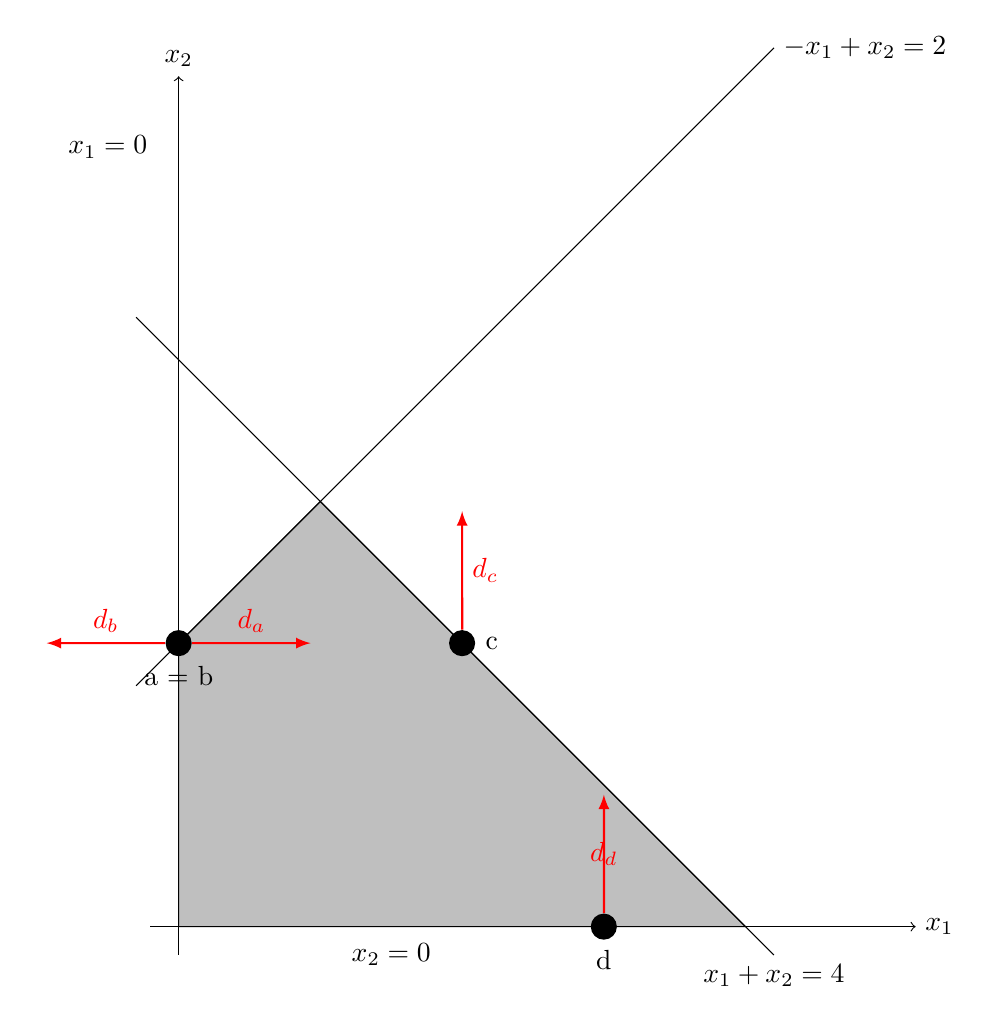
\begin{tikzpicture}[scale=1.8, domain=-0.3:4.2, range=-0.4:6]
  \draw[fill=lightgray]  (0, 0) -- (0, 2) -- (1, 3) -- (4, 0) -- cycle;
  \draw[->] (-0.2, 0) -- (5.2, 0) node[right] {$x_1$};
  \draw[->] (0, -0.2) -- (0, 6) node[above] {$x_2$};
  \draw[color=black] plot (\x, \x+2) node[right] {$-x_1 + x_2 = 2$};
  \draw[color=black] plot (\x, 4-\x) node[below] {$x_1 + x_2 = 4$};
  \node at (1.5, -0.2) {$x_2 = 0$};
  \node at (-0.5, 5.5) {$x_1 = 0$};
  \node (A) at (0, 2) [circle, fill, label=below:{a = b}] {};
  \node (da) at (1, 2) {} ;
  \draw[-latex, color=red, thick] (A) -- (da) node[midway, text=red, above] {$d_a$} ;
  \node (db) at (-1, 2) {} ;
  \draw[-latex, color=red, thick] (A) -- (db) node[midway, text=red, above] {$d_b$} ;
  \node (C) at (2, 2) [circle, fill, label=right:c] {};
  \node (dc) at (2, 3) {} ;
  \draw[-latex, color=red, thick] (C) -- (dc) node[midway, text=red, right] {$d_c$} ;
  \node (D) at (3, 0) [circle, fill, label=below:d] {};
  \node (dd) at (3, 1) {} ;
  \draw[-latex, color=red, thick] (D) -- (dd) node[midway, text=red] {$d_d$} ;
\end{tikzpicture}
